%%%%%%%%%%%%%%%%%%%%%%%%%%%%%%%%%%%%%%%%%%%%%%%%%%%%%%%%%%%%%%%%%%%%%
% LaTeX Template: Project Titlepage Modified (v 0.1) by rcx
%
% Original Source: http://www.howtotex.com
% Date: February 2014
% 
% This is a title page template which be used for articles & reports.
% 
% This is the modified version of the original Latex template from
% aforementioned website.
% 
%%%%%%%%%%%%%%%%%%%%%%%%%%%%%%%%%%%%%%%%%%%%%%%%%%%%%%%%%%%%%%%%%%%%%%

\documentclass[12pt]{report}
\usepackage[a4paper]{geometry}
\usepackage[myheadings]{fullpage}
\usepackage{fancyhdr}
\usepackage{lastpage}
\usepackage{graphicx, wrapfig, subcaption, setspace, booktabs}
\usepackage[T1]{fontenc}
\usepackage[font=small, labelfont=bf]{caption}
\usepackage{fourier}
\usepackage[protrusion=true, expansion=true]{microtype}
\usepackage[english]{babel}
\usepackage{sectsty}
\usepackage{url, lipsum}

%% This turns references into clickable hyperlinks.
\usepackage[bookmarks,backref=true,linkcolor=black]{hyperref} %,colorlinks
\hypersetup{
  pdfauthor = {},
  pdftitle = {},
  pdfsubject = {},
  pdfkeywords = {},
  colorlinks=true,
  linkcolor= black,
  citecolor= black,
  pageanchor=true,
  urlcolor = black,
  plainpages = false,
  linktocpage
}

\newcommand{\HRule}[1]{\rule{\linewidth}{#1}}
\onehalfspacing
\setcounter{tocdepth}{5}
\setcounter{secnumdepth}{5}

%-------------------------------------------------------------------------------
% HEADER & FOOTER
%-------------------------------------------------------------------------------
\pagestyle{fancy}
\fancyhf{}
\setlength\headheight{15pt}
\fancyhead[L]{Jonathan Bosson, Isabell Jansson}
\fancyhead[R]{Link\"oping University}
\fancyfoot[R]{Page \thepage\ of \pageref{LastPage}}
%-------------------------------------------------------------------------------
% TITLE PAGE
%-------------------------------------------------------------------------------

\begin{document}

\title{ \LARGE \textsc{Interactive Equation Solver}
		\\ [1.0cm]
		\normalsize \textbf{\uppercase{Through Neural Network and Optical Character Recognition}}
		\HRule{2pt} \\ [0.5cm]
		\normalsize \today \vspace*{5\baselineskip}}

\date{}

\author{
		Jonathan Bosson \\ 
		Isabell Jansson \\
		Link\"oping University }

\maketitle


\section*{Abstract}
\newpage

\tableofcontents
\newpage

%-------------------------------------------------------------------------------
% Section title formatting
\sectionfont{\scshape}
%-------------------------------------------------------------------------------

%-------------------------------------------------------------------------------
% BODY
%-------------------------------------------------------------------------------

\section*{Introduction}
\addcontentsline{toc}{section}{Introduction}

This paper discusses the theory behind and the implementation of an interactive equation solver which reads an equation from a web camera. The technique, strengths and weaknesses, behind optical character recognition (OCR) and a multilayered perceptron (MLP) neural network are discussed. It also investigates how the computer can understand and solve an equation through training with a  dataset of digital characters in handwritten-esque. All of these methods, apart from the precomputed training, are computationally fast and are done in real-time in the application.



\section*{Theory}
\addcontentsline{toc}{section}{Theory}

\subsection*{Multilayered perceptron neural network}
\addcontentsline{toc}{subsection}{Multilayered perceptron neural network}

The MLP is a neural network that consists of three layers; the input layer, the hidden layer and the output layer.  It is a feed forward neural network, which means that each layer consists of neurons that are linked with the neurons of the next layer, as illustrated in Figure \ref{fig:layers} below.

\begin{figure}[!ht]
	\centering
	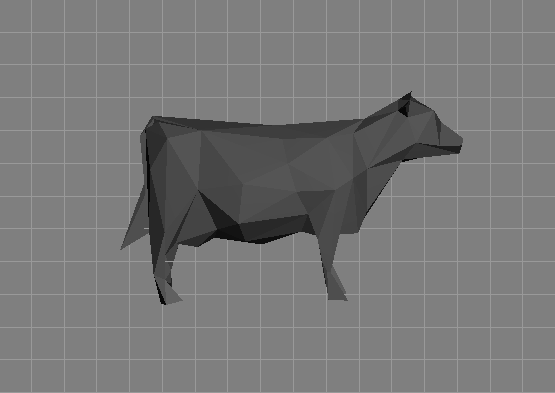
\includegraphics[width=0.6\textwidth]{figure.png}
	\caption{\label{fig:layers} some text about it}
	\centering
\end{figure}
The input values for a layer are summed up with certain weights that are specific for every neuron together with a bias term. This represents the decision that the neuron will take. The weights are calculated by a weight-function, which can be seen in Equation \ref{eq:weight} below. In the equation, $u_i$ is the total input for the layer, $x_j$  is the neuron which will be weighted with $w_{ij}$ , $n$ is the current layer and  $w_i$, bias is the bias term for the neuron \cite{mlp}. 

\begin{equation}
  \label{eq:weight}
  u_i = \sum_j^n (w_{i,j}^{n+1} \ \cdot \ x_j) \ + \ w_{i,bias}^{n+1}
\end{equation}
The weight for each neuron is determined by the training algorithm. OpenCV offers two versions of backpropagation as the training algorithm, standard backpropagation and the rprop algorithm which is a direct adaptive method for faster backpropagation learning. The standard backpropagation algorithm, which is used in this project, is the most widely used supervised training method for neural networks. It takes a set of inputs and outputs, $(x_1, y_1)...(x_n,y_n)$, and outputs a sequence of weights. These weights are initially set randomly but are updated during the training. This is done by calculating the gradient of a loss function with respect to all weights in the network. The gradient is used into an optimization method which uses the gradient to update the weights in order to minimize the loss function. 
\newline
\newline
An activation function is then used to transform the ui into the output of the layer, which will be used as the input in the next. The activation function used in this project is the Sigmoid function, which is default in MLP in OpenCV and can be seen in Equation \ref{eq:activate}. In the equation a and b are constants and ui is the input of the layer calculated according to Equation \ref{eq:activate}.


\begin{equation}
  \label{eq:activate}
  f(u_i) = \beta \ \cdot \ \frac{(1-e^{-au_i})}{1+e^{-au_i})}
\end{equation}



\section*{Method}
\addcontentsline{toc}{section}{Method}

The project contains three parts:

\begin{itemize}  
\item \textbf{Preporcessing} -  Each image in the dataset contains a character which is converted into a string of bits by thresholding the image. The image is then cropped and rescaled before storing the result into a text file and which is used in the following step. 
\item \textbf{Training} - The processed dataset is used as the input for the training of the MLP-neural network. The result is exported and used in the application.
\item \textbf{Application} - The application uses a web camera to register characters. The neural network is guessing the classification of the characters in each frame. If the registered characters define a valid mathematical expression, the application is calculating the result of the expression and dispose it to the user. \ldots 
\end{itemize}



\subsection*{Preprocessing training set}
\addcontentsline{toc}{subsection}{Preprocessing training set}

The dataset contains sample images of the characters $0-9, y, x, D , A, S, E$ which are a part of the $Char74K$ dataset \cite{dataset}. The characters $x, D, A, S$ and $E$ are used for multiplication, division, addition and subtraction respectively and y is used as the unknown character which will be solved from the equation. Letters were used as operators since no free database with $+,-,/$ and $=$ could be found. It has also been tested to create a smaller dataset of seven images of each operator. To still be able to have a bigger dataset for the remaining characters, the algorithm require that all characters have the same amount of training images, white image was used for training the operators when the seven images were done. Since the algorithm will match a character to the most equal one, the empty images will always be less equal to the input then the first seven.  
\newline
\newline
The dataset contains $1016$ different computer font images of each character where every image is a $128*128$ PNG-image. A part of the dataset is used for training and the remaining images are used for testing the result of the training. The amount of images for each characters that were used for training was varied, see Table \ref{table}.
\newline
\newline
The original code for the preprocessing is written by Kristoffer Janukiewicz \cite{preprocessing}. Every sample for all characters are preprocessed into a binary string which is a valuable input for the neural network. Since the project uses $16$ different characters, the maximum amount of images to preprocess is $16*1016 = 16256$, assuming that all images are used for training. Noise is removed by thresholding the images and the images will be converted into binary images. The images are cropped by finding the most upper, rightmost, downwards and leftmost one in the binary image. The cropped image is rescaled into a small patch. The patch sizes have been varied between $8*8$, $16*16$ and $32*32$. The patch is then stored as a string of zeros and ones. 


\subsection*{Train network}
\addcontentsline{toc}{subsection}{Train network}

The MLP neural network in this project contains three layers. The amount of neurons in each layer in this project is:

\begin{itemize}  
\item \textbf{Input layer:} The size of all dimensions in an input patch (E.g. a $16*16$ patch gives an input layer of $256$ neurons).
\item \textbf{Hidden layer:} The size of one dimension of the input patch (E.g. a $16*16$ patch gives a hidden layer of $16$ neurons).
\item \textbf{Output layer:} The amount of characters that have to be classified (E.g. $0-9, y, x, A, S, D, E$ are $16$ characters which gives an output layer of $16$ neurons). 
\end{itemize}
The training were performed using OpenCV with the Sigmoid function as activation function. The values for $\alpha$ and $\beta$ were set to $0.6$ and $1.0$ respectively. The weights are calculated by backpropagation, which also is included into OpenCV. The training will end after a maximum of $1000$ iterations or when the error of the loss function is less than $10^{-6}$. For predicting the class of a character, either from the testing set or from the application, the character will be matched to all output classes and the result will be described by a weight. The class corresponding to the highest weight will be the resulting output, which is the decision of the neural network. The result of the training is stored into an XML-file which is imported into the application. 


\subsection*{Application}
\addcontentsline{toc}{subsection}{Application}

The application uses the webcam, finds the characters on the screen, predicts their values and calculates the result. The training from the previous stage is loaded into the application from an XML-file. Since the program is run in real-time are some restrictions required concerning the image processing. The frame goes through four steps of filters. Grayscaling the image, applying a Sobel filter to find high intensity areas and highlighting the contours, Otsu's threshold filter to remove noise and lastly a morphology dilation to fill in gaps to improve the recognition. After that can OpenCV accurately extract where in the frame a character exists and predict it with the network. A more detailed description of the image processing and character search can be read in Kristofer Janukiewicz paper \cite{kristofer}.
\newline
\newline
All characters that has been found in the frame are sorted from left to right to later be sent into the equation solver. Since the solver will receive a new expression in each frame it is important to check if it is a valid expression, else it would quickly cause a crash of the program. The expression has to be valid such that it doesn't include multiple equals signs, multiple operators after each other as well as start and end with an operand. Once through the validation the expression is translated to a stack principle like Equation \ref{eq:1}.

\begin{equation}
  \label{eq:1}
  \overbrace{ y \cdot 2+\frac{5}{2}=10-3 \cdot 2}^{original \ expression} \ \ \to \ \ \underbrace{y,2,\cdot,5,2,\div,+,=10,3,2,\cdot,-}_{stack \ expression}
\end{equation}
The operands are placed on top of the stack followed by an operator. The precedence is respected by placing the preceding operator on top of the other on the stack. The expression is then split into three parts, $C$, $L$ and $R$. $C$ is the opposing side of where the $y$ exists, $L$ is the left side of the variable and $R$ the right side.

\begin{equation}
  \label{eq:2}
  \overbrace{}^{L}y, \underbrace{2, \cdot ,5,2,\div,+}_{R} \ = \ \overbrace{10,3,2, \cdot ,-}^{C} \ \ \to \ \ y \ = \ C,L,-,R'
\end{equation}
If the expression does not include any equal sign or variable are $L$ and $R$ both equal to $0$. The $C$ and $L$ can be computed separately due to the structure of the stack. The original equation is then reordered such that the variable is empty on one side, like Equation \ref{eq:2}. The operators in the $R$-part requires to be looked over, however in what way depends on the structure of the original expression. Addition and subtraction operators are inverted while multiplication and division kept the same. If the very first operator in $R$ is either multiplication or division will that one be inverted as well but placed at the bottom of the stack together with its operand. This process is repeated until an addition or subtraction operator is found. If the variable was negative will the computed result be divided by $-1$. Equation \ref{eq:1} will turn into:

\begin{equation}
  \label{eq:3}
  C,L,-,R' \ \ \iff \ \  \overbrace{10,3,2,\cdot,-}^{C \ = \ 4},\underbrace{0}_{L},-,\overbrace{5,2,\div,-,2,\div}^{R'} \ \ \iff \ \ \frac{(4-\frac{5}{2})}{2} \ \ \iff \ \ \frac{3}{4} \ = \ y
\end{equation}


\section*{Implementation}
\addcontentsline{toc}{section}{Implementation}

The project is developed in C++ with OpenCV 3.1.0 \cite{opencv}. A Multi-Layered Perceptron neural network was used for machine learning, which is included in OpenCV.  The code is compiled with the GNU C++ Compiler with OpenCV flags.  The character images are downloaded from the Chars74K dataset \cite{dataset}.


\section*{Results}
\addcontentsline{toc}{section}{Results}

The results when using a testing set to test the neural network can be found in Table \ref{table} below. The result when running the actual application varied a lot. Two snapshots from the application can be seen in Figure \ref{fig:result}.

\begin{figure}[!ht]
	\centering
	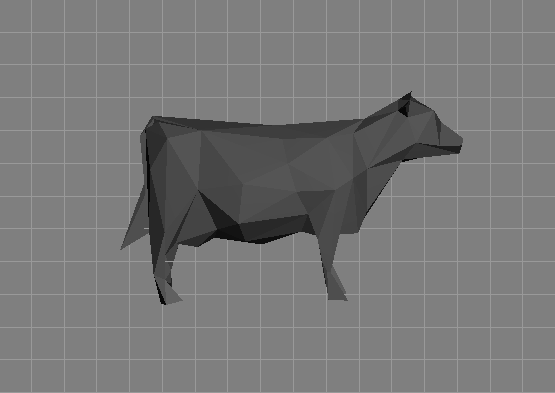
\includegraphics[width=0.6\textwidth]{figure.png}
	\caption{\label{fig:result} Snapshots from the application}
	\centering
\end{figure}

% Maybe take away comments?
\begin{table}[]
\centering
\resizebox{\textwidth}{!}{%
\begin{tabular}{clrrr}
\textbf{Patch size} & \textbf{Comments} & \begin{tabular}[c]{@{}l@{}}\textbf{Training set}\\ \textbf{(pictures per class)}\end{tabular} & \begin{tabular}[c]{@{}l@{}}\textbf{Test set} \\ \textbf{(pictures per class)}\end{tabular} & \textbf{Correct guess} \\ \\
$8*8$ & \begin{tabular}[c]{@{}l@{}}Dataset contains handwritten characters. \\
Using characters $+,-,/,=$ as operators\end{tabular} & $3$ & $3$ & $64\%$ \\ \\
$8*8$ & \begin{tabular}[c]{@{}l@{}}Dataset contains handwritten characters. \\
Using characters $+,-,/,=$ as operators.\end{tabular} & $52$ ($7$ for operators) & $3$ & $66\%$ \\ \\
$8*8$ & \begin{tabular}[c]{@{}l@{}}Dataset contains computer fonts. \\
Using characters $+,-,/,=$ as operators.\end{tabular} & $1013$ ($7$ for operators) & $3$ & $66\%$ \\ \\
$8*8$ & \begin{tabular}[c]{@{}l@{}}Dataset contains computer fonts. \\
Using characters $A,S,D,E$ as operators.\end{tabular} & $916$ & $100$ & $91\%$ \\ \\
$16*16$ & \begin{tabular}[c]{@{}l@{}}Dataset contains handwritten characters. \\
Using characters $+,-,/,=$ as operators.\end{tabular} & $3$ & $3$ & $89\%$ \\ \\
$16*16$ & \begin{tabular}[c]{@{}l@{}}Dataset contains handwritten characters. \\
Using characters $+,-,/,=$ as operators.\end{tabular} & $52$ ($7$ for operators) & $3$ & $85\%$ \\ \\
$16*16$ & \begin{tabular}[c]{@{}l@{}}Dataset contains computer fonts. \\
Using characters $+,-,/,=$ as operators.\end{tabular} & $1013$ ($7$ for operators) & $3$ & $62\%$ \\ \\
$16*16$ & \begin{tabular}[c]{@{}l@{}}Dataset contains computer fonts. \\
Using characters $A,S,D,E$ as operators.\end{tabular} & $916$ & $100$ & $96\%$ \\ \\
$32*32$ & \begin{tabular}[c]{@{}l@{}}Dataset contains handwritten characters. \\
Using characters $+,-,/,=$ as operators.\end{tabular} & $3$ & $3$ & $81\%$ \\ \\
$32*32$ & \begin{tabular}[c]{@{}l@{}}Dataset contains handwritten characters. \\
Using characters $+,-,/,=$ as operators.\end{tabular} & $52$ ($7$ for operators) & $3$ & $89\%$ \\ \\
$32*32$ & \begin{tabular}[c]{@{}l@{}}Dataset contains computer fonts. \\
Using characters $+,-,/,=$ as operators.\end{tabular} & $1013$ ($7$ for operators) & $3$ & $77\%$ \\ \\
$32*32$ & \begin{tabular}[c]{@{}l@{}}Dataset contains computer fonts. \\
Using characters $A,S,D,E$ as operators.\end{tabular} & $916$ & $100$ & $98\%$
\end{tabular}%
}
\caption{\label{table} Results from training}

\end{table}

\section*{Discussion and conclusion}
\addcontentsline{toc}{section}{Discussion and conclusion}

The biggest contributing factors for errors in the character predictions are the quality of the webcam as well as the light settings in the room when the application is running. The better the original picture the better will the recognition work. In the development of this application was five years old integrated laptop webcams used in a gloomy lit room. This results in more noise in an order of magnitude, making Otsu's threshold filter not enough to remove all outlines but the contours from the characters. Slight orientation differences between the camera and the paper on which the characters are written can also affect prediction accuracy in a big way. Another issue is the MLP neural network as it has troubles identifying this many different characters, especially since many of them share a lot of similarities. A idea could be to change the number of hidden layers, however it can be difficult to find the optimal number. If the data is linearly separable then hidden layers are not needed, and even if not is the improved performance negligible in most applications. 
\newline
\newline
The MLP uses a backpropagation algorithm to train, as is the standard for any supervised learning. There is an application developed by Alistar Dobke and Mark Mann which is also using a feed forward MLP neural network but trained with a conjugate scaled gradient backpropagation. The application is developed for mobile Android devices and is a simple calculator as it only contains the addition and subtraction operators and no variable. Though the application is simpler than the application developed in this project, it seems to have achieved more reliable results \cite{app}, however it were unable to prove since the application was unresponsive. Using another training set could also make handwritten character predictions more reliable. This was clear after seeing the improvement by swapping from a small dataset of handwritten characters to a much larger one with computer written characters. The result from the test set will vary depending on the size of the training set. If a small training set is used, it is likely that the training set will not be a good representation of the real data set. Since if the training set is small, a wrong classification has a bigger impact on the result which is the case when using only three testing images. A $2\%$ increase were achieved in accuracy using $32*32$ patch size over $16*16$, although that improvement is rather small compared to the improvement between $16*16$ and $8*8$ patch sizes. Using $32*32$ is four times as computationally heavy as $16*16$, however since the training is only done once and not tied to the output application is that irrelevant to the user. 
\newline
\newline
The prediction of the MLP neural network can be improved in numerous different ways, mainly targeted at the training techniques. For best results, it is recommended to have a high quality camera and a well lit room when using the application. The application can effectively find characters on an even surface and, as long as the prediction is correct, has no trouble calculating the given expression.



%-------------------------------------------------------------------------------
% REFERENCES
%-------------------------------------------------------------------------------
\newpage
\renewcommand{\bibname}{}
\begin{thebibliography}{}
\section*{References}
\addcontentsline{toc}{section}{References}

\bibitem{mlp} Multilayered perceptron neural network, \url{http://docs.opencv.org/2.4/modules/ml/doc/neural_networks.html}, 2016-10-28

\bibitem{dataset} The Chars74K image dataset, T.deCampos, \url{http://www.ee.surrey.ac.uk/CVSSP/demos/chars74k/}, 2016-09-28 

\bibitem{preprocessing} Preprocessing of the dataset, Kristoffer Janukiewics,  
\url{https://github.com/KristoferJanukiewicz/Neural-Network-Approach-for-Optical-Character-Recognition/blob/master/Preprocessing.cpp}, 2016-10-11 

\bibitem{kristofer} Neural Network, Multi-Layered Perceptron, Image Processing and Computer Vision, Kristofer Janukiewicz, \url{http://weber.itn.liu.se/~piede/courses/tnm095/archive/2015/p2.pdf}, 2015-11-09

\bibitem{opencv} OpenCV 3.1.0, OpenCV Dev. Team, \url{http://docs.opencv.org/3.1.0/index.html}, 2016-10-11

\bibitem{app} OCR for Mathematical Expressions, Alistar Dobke and Mark Mann, \url{https://www.cs.hmc.edu/~adobke/nn/}, Fall 2012


\end{thebibliography}


\end{document}

%-------------------------------------------------------------------------------
% SNIPPETS
%-------------------------------------------------------------------------------

%\begin{figure}[!ht]
%	\centering
%	\includegraphics[width=0.8\textwidth]{file_name}
%	\caption{}
%	\centering
%	\label{label:file_name}
%\end{figure}

%\begin{figure}[!ht]
%	\centering
%	\includegraphics[width=0.8\textwidth]{graph}
%	\caption{Blood pressure ranges and associated level of hypertension (American Heart Association, 2013).}
%	\centering
%	\label{label:graph}
%\end{figure}

%\begin{wrapfigure}{r}{0.30\textwidth}
%	\vspace{-40pt}
%	\begin{center}
%		\includegraphics[width=0.29\textwidth]{file_name}
%	\end{center}
%	\vspace{-20pt}
%	\caption{}
%	\label{label:file_name}
%\end{wrapfigure}

%\begin{wrapfigure}{r}{0.45\textwidth}
%	\begin{center}
%		\includegraphics[width=0.29\textwidth]{manometer}
%	\end{center}
%	\caption{Aneroid sphygmomanometer with stethoscope (Medicalexpo, 2012).}
%	\label{label:manometer}
%\end{wrapfigure}

%\begin{table}[!ht]\footnotesize
%	\centering
%	\begin{tabular}{cccccc}
%	\toprule
%	\multicolumn{2}{c} {Pearson's correlation test} & \multicolumn{4}{c} {Independent t-test} \\
%	\midrule	
%	\multicolumn{2}{c} {Gender} & \multicolumn{2}{c} {Activity level} & \multicolumn{2}{c} {Gender} \\
%	\midrule
%	Males & Females & 1st level & 6th level & Males & Females \\
%	\midrule
%	\multicolumn{2}{c} {BMI vs. SP} & \multicolumn{2}{c} {Systolic pressure} & \multicolumn{2}{c} {Systolic Pressure} \\
%	\multicolumn{2}{c} {BMI vs. DP} & \multicolumn{2}{c} {Diastolic pressure} & \multicolumn{2}{c} {Diastolic pressure} \\
%	\multicolumn{2}{c} {BMI vs. MAP} & \multicolumn{2}{c} {MAP} & \multicolumn{2}{c} {MAP} \\
%	\multicolumn{2}{c} {W:H ratio vs. SP} & \multicolumn{2}{c} {BMI} & \multicolumn{2}{c} {BMI} \\
%	\multicolumn{2}{c} {W:H ratio vs. DP} & \multicolumn{2}{c} {W:H ratio} & \multicolumn{2}{c} {W:H ratio} \\
%	\multicolumn{2}{c} {W:H ratio vs. MAP} & \multicolumn{2}{c} {\% Body fat} & \multicolumn{2}{c} {\% Body fat} \\
%	\multicolumn{2}{c} {} & \multicolumn{2}{c} {Height} & \multicolumn{2}{c} {Height} \\
%	\multicolumn{2}{c} {} & \multicolumn{2}{c} {Weight} & \multicolumn{2}{c} {Weight} \\
%	\multicolumn{2}{c} {} & \multicolumn{2}{c} {Heart rate} & \multicolumn{2}{c} {Heart rate} \\
%	\bottomrule
%	\end{tabular}
%	\caption{Parameters that were analysed and related statistical test performed for current study. BMI - body mass index; SP - systolic pressure; DP - diastolic pressure; MAP - mean arterial pressure; W:H ratio - waist to hip ratio.}
%	\label{label:tests}
%\end{table}